\documentclass[11pt,a4paper]{article}
\usepackage[a4paper,margin=0.75in]{geometry}
\usepackage{amsmath,amssymb,mathtools}
\usepackage{tikz}
\usetikzlibrary{arrows.meta,calc,patterns,positioning}
\usepackage{array,booktabs,longtable,multicol}
\usepackage{enumitem}
\usepackage{xcolor}
\usepackage{fancyhdr}
\usepackage{tcolorbox}
\usepackage[hidelinks]{hyperref}
\setlength{\parindent}{0pt}
\setlength{\parskip}{5pt}
\pagestyle{fancy}
\fancyhf{}
\lhead{BCS-012 Basic Mathematics}
\rhead{June 2023 Solved Paper}
\cfoot{\thepage}
\definecolor{myblue}{HTML}{153E75}
\definecolor{lightblue}{HTML}{EAF3FF}
\newtcolorbox{questionbox}{colback=lightblue,colframe=myblue,boxrule=0.6pt,arc=2mm,left=1mm,right=1mm,top=1mm,bottom=1mm}
\newcommand{\ans}{\textbf{Solution.} }
\newcommand{\final}[1]{\[\boxed{#1}\]}
\begin{document}
\begin{center}
{\Large\bfseries IGNOU BCS-012: Basic Mathematics}\\[2mm]
{\large\bfseries Term-End Examination, June 2023 -- Solved Paper}\\[1mm]
Time: 3 Hours \qquad Maximum Marks: 100
\end{center}

\begin{questionbox}
\textbf{Note.} Question Number 1 is compulsory. Attempt any three questions from the remaining questions.
\end{questionbox}

\section*{Question 1}

\subsection*{1(a)}
\begin{questionbox}
If
\[
A=\begin{bmatrix}1&-2\\2&-1\end{bmatrix},\qquad
B=\begin{bmatrix}a&1\\ b&-1\end{bmatrix}
\]
and $(A+B)^2=A^2+B^2$, find $a$ and $b$.
\end{questionbox}
\ans
Since
\[
(A+B)^2=A^2+AB+BA+B^2,
\]
the given condition implies
\[
AB+BA=O.
\]
Now
\[
AB=\begin{bmatrix}1&-2\\2&-1\end{bmatrix}
\begin{bmatrix}a&1\\b&-1\end{bmatrix}
=
\begin{bmatrix}a-2b&3\\2a-b&3\end{bmatrix},
\]
and
\[
BA=\begin{bmatrix}a&1\\b&-1\end{bmatrix}
\begin{bmatrix}1&-2\\2&-1\end{bmatrix}
=
\begin{bmatrix}a+2&-2a-1\\b-2&-2b+1\end{bmatrix}.
\]
Therefore
\[
AB+BA=\begin{bmatrix}
2a-2b+2&2-2a\\2a-2&4-2b
\end{bmatrix}=O.
\]
Thus $2-2a=0$ and $4-2b=0$, giving
\final{a=1,\quad b=2.}

\subsection*{1(b)}
\begin{questionbox}
Show that $n(n+1)(2n+1)$ is a multiple of $6$ for every natural number $n$.
\end{questionbox}
\ans
We need to prove divisibility by $2$ and by $3$.

Among $n$ and $n+1$, one is even. Hence $n(n+1)(2n+1)$ is divisible by $2$.

For divisibility by $3$, consider three cases:
\begin{itemize}[leftmargin=*]
\item If $n\equiv 0\pmod 3$, then $n$ is divisible by $3$.
\item If $n\equiv 2\pmod 3$, then $n+1\equiv 0\pmod 3$.
\item If $n\equiv 1\pmod 3$, then $2n+1\equiv 2(1)+1=3\equiv 0\pmod 3$.
\end{itemize}
So the product is divisible by $3$. Since it is divisible by both $2$ and $3$, it is divisible by $6$.
\final{6\mid n(n+1)(2n+1)}

\subsection*{1(c)}
\begin{questionbox}
If $1,\omega,\omega^2$ are cube roots of unity, show that
\[
(2-\omega)(2-\omega^2)(2-\omega^{10})(2-\omega^{11})=49.
\]
\end{questionbox}
\ans
For cube roots of unity,
\[
\omega^3=1,\qquad 1+\omega+\omega^2=0.
\]
Hence
\[
\omega^{10}=\omega^{9}\omega=\omega,
\qquad
\omega^{11}=\omega^9\omega^2=\omega^2.
\]
So
\[
(2-\omega)(2-\omega^2)(2-\omega^{10})(2-\omega^{11})
=\{(2-\omega)(2-\omega^2)\}^2.
\]
Now
\[
(2-\omega)(2-\omega^2)=4-2(\omega+\omega^2)+\omega^3
=4-2(-1)+1=7.
\]
Therefore
\final{(2-\omega)(2-\omega^2)(2-\omega^{10})(2-\omega^{11})=7^2=49.}

\subsection*{1(d)}
\begin{questionbox}
Show that $|\vec a|\vec b+|\vec b|\vec a$ is perpendicular to $|\vec a|\vec b-|\vec b|\vec a$, for any two non-zero vectors $\vec a$ and $\vec b$.
\end{questionbox}
\ans
Let
\[
\vec u=|\vec a|\vec b+|\vec b|\vec a,
\qquad
\vec v=|\vec a|\vec b-|\vec b|\vec a.
\]
Then
\[
\vec u\cdot\vec v
=(|\vec a|\vec b+|\vec b|\vec a)\cdot(|\vec a|\vec b-|\vec b|\vec a).
\]
Using the identity $(p+q)\cdot(p-q)=p\cdot p-q\cdot q$,
\[
\vec u\cdot\vec v
=|\vec a|^2(\vec b\cdot\vec b)-|\vec b|^2(\vec a\cdot\vec a)
=|\vec a|^2|\vec b|^2-|\vec b|^2|\vec a|^2=0.
\]
Therefore the two vectors are perpendicular.
\final{\vec u\perp\vec v}

\subsection*{1(e)}
\begin{questionbox}
Solve the equation $2x^3-15x^2+37x-30=0$, given that the roots of the equation are in A.P.
\end{questionbox}
\ans
Since the roots are in A.P., let them be $a-d,a,a+d$.
For the cubic equation
\[
2x^3-15x^2+37x-30=0,
\]
the sum of the roots is
\[
\frac{15}{2}.
\]
Thus
\[
(a-d)+a+(a+d)=3a=\frac{15}{2}
\quad\Rightarrow\quad
 a=\frac{5}{2}.
\]
So one root is $\frac{5}{2}$. Dividing the polynomial by $x-\frac{5}{2}$, or equivalently by $2x-5$, we get
\[
2x^3-15x^2+37x-30=(2x-5)(x^2-5x+6).
\]
Now
\[
x^2-5x+6=(x-2)(x-3).
\]
Hence
\final{x=2,\quad \frac{5}{2},\quad 3.}

\subsection*{1(f)}
\begin{questionbox}
Evaluate the integral
\[
I=\int \frac{x^2}{(x+1)^3}\,dx.
\]
\end{questionbox}
\ans
Put $u=x+1$. Then $x=u-1$ and $dx=du$.
\[
I=\int \frac{(u-1)^2}{u^3}\,du
=\int \frac{u^2-2u+1}{u^3}\,du.
\]
Thus
\[
I=\int\left(\frac1u-\frac{2}{u^2}+\frac1{u^3}\right)du.
\]
Integrating term by term,
\[
I=\ln|u|+\frac{2}{u}-\frac{1}{2u^2}+C.
\]
Putting $u=x+1$,
\final{I=\ln|x+1|+\frac{2}{x+1}-\frac{1}{2(x+1)^2}+C.}

\subsection*{1(g)}
\begin{questionbox}
Use first derivative test to find the local maxima and local minima if $f(x)=x^3-12x$.
\end{questionbox}
\ans
\[
f(x)=x^3-12x,
\qquad
f'(x)=3x^2-12=3(x-2)(x+2).
\]
Critical points are
\[
x=-2,\quad x=2.
\]
Sign of $f'(x)$:
\[
\begin{array}{c|ccc}
\text{Interval} & (-\infty,-2)&(-2,2)&(2,\infty)\\\hline
f'(x)&+&-&+
\end{array}
\]
Hence the function changes from increasing to decreasing at $x=-2$, so there is a local maximum.
It changes from decreasing to increasing at $x=2$, so there is a local minimum.
\[
f(-2)=(-2)^3-12(-2)=16,
\qquad
f(2)=8-24=-16.
\]
\final{\text{Local maximum }=(-2,16),\qquad \text{local minimum }=(2,-16).}

\begin{center}
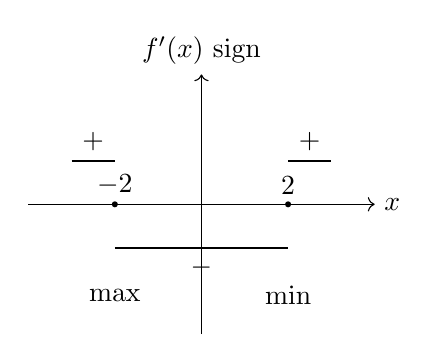
\begin{tikzpicture}[scale=0.55]
\draw[->] (-4,0)--(4,0) node[right] {$x$};
\draw[->] (0,-3)--(0,3) node[above] {$f'(x)$ sign};
\draw[thick] (-3,1)--(-2,1) node[midway,above] {$+$};
\draw[thick] (-2,-1)--(2,-1) node[midway,below] {$-$};
\draw[thick] (2,1)--(3,1) node[midway,above] {$+$};
\fill (-2,0) circle (2pt) node[above] {$-2$};
\fill (2,0) circle (2pt) node[above] {$2$};
\node at (-2,-2.1) {max};
\node at (2,-2.1) {min};
\end{tikzpicture}
\end{center}

\subsection*{1(h)}
\begin{questionbox}
Prove that the three medians of a triangle meet at a point called centroid and divide each of the medians in the ratio $2:1$.
\end{questionbox}
\ans
Let the vertices of the triangle be
\[
A(x_1,y_1),\quad B(x_2,y_2),\quad C(x_3,y_3).
\]
The midpoint of $BC$ is
\[
D\left(\frac{x_2+x_3}{2},\frac{y_2+y_3}{2}\right).
\]
The point which divides median $AD$ in the ratio $2:1$ from $A$ to $D$ is
\[
G=\left(\frac{x_1+x_2+x_3}{3},\frac{y_1+y_2+y_3}{3}\right).
\]
Similarly, the midpoint of $CA$ and the midpoint of $AB$ give the same point $G$ on the other two medians. Hence all three medians pass through the same point
\[
G\left(\frac{x_1+x_2+x_3}{3},\frac{y_1+y_2+y_3}{3}\right).
\]
This common point is called the centroid. Since $G$ divides each median in the ratio $2:1$ from the vertex, the result is proved.

\begin{center}
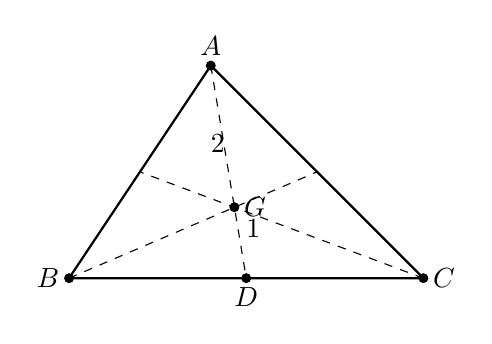
\begin{tikzpicture}[scale=0.9]
\coordinate (A) at (0,3);
\coordinate (B) at (-2,0);
\coordinate (C) at (3,0);
\coordinate (D) at ($(B)!0.5!(C)$);
\coordinate (E) at ($(A)!0.5!(C)$);
\coordinate (F) at ($(A)!0.5!(B)$);
\coordinate (G) at ($(A)!0.666!(D)$);
\draw[thick] (A)--(B)--(C)--cycle;
\draw[dashed] (A)--(D);
\draw[dashed] (B)--(E);
\draw[dashed] (C)--(F);
\fill (A) circle (2pt) node[above] {$A$};
\fill (B) circle (2pt) node[left] {$B$};
\fill (C) circle (2pt) node[right] {$C$};
\fill (D) circle (2pt) node[below] {$D$};
\fill (G) circle (2pt) node[right] {$G$};
\node at (0.1,1.9) {$2$};
\node at (0.6,0.7) {$1$};
\end{tikzpicture}
\end{center}

\section*{Question 2}

\subsection*{2(a)}
\begin{questionbox}
Verify that $2+2^2+\cdots+2^n=2^{n+1}-2$ using the principle of mathematical induction.
\end{questionbox}
\ans
For $n=1$,
\[
\text{LHS}=2,
\qquad
\text{RHS}=2^{2}-2=2.
\]
So the result is true for $n=1$.

Assume it is true for $n=k$:
\[
2+2^2+\cdots+2^k=2^{k+1}-2.
\]
For $n=k+1$,
\[
2+2^2+\cdots+2^k+2^{k+1}
=(2^{k+1}-2)+2^{k+1}
=2\cdot 2^{k+1}-2
=2^{k+2}-2.
\]
This is the required formula for $k+1$. Hence, by induction,
\final{2+2^2+\cdots+2^n=2^{n+1}-2.}

\subsection*{2(b)}
\begin{questionbox}
Determine the 10th term of the Harmonic Progression
\[
\frac17,\frac1{15},\frac1{23},\ldots.
\]
\end{questionbox}
\ans
The reciprocals of an H.P. form an A.P. Thus
\[
7,15,23,\ldots
\]
is an A.P. with first term $a=7$ and common difference $d=8$.
The 10th term of this A.P. is
\[
T_{10}=a+9d=7+9(8)=79.
\]
Therefore, the 10th term of the original H.P. is
\final{\frac1{79}.}

\subsection*{2(c)}
\begin{questionbox}
Evaluate
\[
\int \frac{dx}{\sqrt{x}+x}.
\]
\end{questionbox}
\ans
Put $t=\sqrt{x}$. Then $x=t^2$ and $dx=2t\,dt$.
\[
\int \frac{dx}{\sqrt{x}+x}
=\int \frac{2t\,dt}{t+t^2}
=\int \frac{2t\,dt}{t(1+t)}
=\int \frac{2}{1+t}\,dt.
\]
Therefore
\[
\int \frac{dx}{\sqrt{x}+x}=2\ln|1+t|+C.
\]
Putting $t=\sqrt{x}$,
\final{\int \frac{dx}{\sqrt{x}+x}=2\ln|1+\sqrt{x}|+C.}

\subsection*{2(d)}
\begin{questionbox}
Solve the system of equations using Cramer's rule:
\[
x+2y+2z=3,\qquad 3x-2y+z=4,
\qquad x+y+z=2.
\]
\end{questionbox}
\ans
The coefficient determinant is
\[
\Delta=\begin{vmatrix}1&2&2\\3&-2&1\\1&1&1\end{vmatrix}=5.
\]
Replacing the first, second and third columns by constants respectively,
\[
\Delta_x=\begin{vmatrix}3&2&2\\4&-2&1\\2&1&1\end{vmatrix}=5,
\]
\[
\Delta_y=\begin{vmatrix}1&3&2\\3&4&1\\1&2&1\end{vmatrix}=0,
\]
\[
\Delta_z=\begin{vmatrix}1&2&3\\3&-2&4\\1&1&2\end{vmatrix}=5.
\]
By Cramer's rule,
\[
x=\frac{\Delta_x}{\Delta}=1,
\quad
 y=\frac{\Delta_y}{\Delta}=0,
\quad
 z=\frac{\Delta_z}{\Delta}=1.
\]
\final{x=1,\quad y=0,\quad z=1.}

\section*{Question 3}

\subsection*{3(a)}
\begin{questionbox}
Given
\[
x=a+b,
\qquad y=a\omega+b\omega^2,
\qquad z=a\omega^2+b\omega,
\]
verify that $xyz=a^3+b^3$, where $\omega$ is a cube root of unity and $\omega\ne1$.
\end{questionbox}
\ans
For cube roots of unity,
\[
1+\omega+\omega^2=0,
\qquad \omega^3=1.
\]
Now
\[
yz=(a\omega+b\omega^2)(a\omega^2+b\omega).
\]
Therefore
\[
yz=a^2\omega^3+ab(\omega^2+\omega^4)+b^2\omega^3.
\]
Since $\omega^3=1$ and $\omega^4=\omega$,
\[
yz=a^2+b^2+ab(\omega+\omega^2)=a^2+b^2-ab.
\]
Thus
\[
xyz=(a+b)(a^2-ab+b^2)=a^3+b^3.
\]
\final{xyz=a^3+b^3.}

\subsection*{3(b)}
\begin{questionbox}
Given
\[
A=\begin{bmatrix}1&2&2\\2&1&2\\2&2&1\end{bmatrix},
\]
perform the following:
\begin{enumerate}[label=(\roman*)]
\item Determine $A^{-1}$ and $A^3$.
\item Verify that $A^2-4A-5I_3=O$.
\end{enumerate}
\end{questionbox}
\ans
Using elementary operations or the adjoint method,
\[
A^{-1}=\frac15
\begin{bmatrix}
-3&2&2\\2&-3&2\\2&2&-3
\end{bmatrix}.
\]
Also,
\[
A^2=\begin{bmatrix}9&8&8\\8&9&8\\8&8&9\end{bmatrix}.
\]
Hence
\[
A^2-4A-5I_3
=
\begin{bmatrix}9&8&8\\8&9&8\\8&8&9\end{bmatrix}
-
\begin{bmatrix}4&8&8\\8&4&8\\8&8&4\end{bmatrix}
-
\begin{bmatrix}5&0&0\\0&5&0\\0&0&5\end{bmatrix}=O.
\]
Thus the identity is verified.

Further,
\[
A^3=A\cdot A^2
=\begin{bmatrix}
41&42&42\\42&41&42\\42&42&41
\end{bmatrix}.
\]
\final{A^{-1}=\frac15\begin{bmatrix}-3&2&2\\2&-3&2\\2&2&-3\end{bmatrix},\quad
A^3=\begin{bmatrix}41&42&42\\42&41&42\\42&42&41\end{bmatrix}.}

\subsection*{3(c)}
\begin{questionbox}
If the roots of $ax^3+bx^2+cx+d=0$ are in A.P., show that
\[
2b^3-9abc+27a^2d=0.
\]
\end{questionbox}
\ans
Let the roots be
\[
r-s,\quad r,
\quad r+s.
\]
For the cubic $ax^3+bx^2+cx+d=0$,
\[
(r-s)+r+(r+s)=3r=-\frac{b}{a}.
\]
Thus
\[
r=-\frac{b}{3a}.
\]
The product of the roots is
\[
(r-s)r(r+s)=r(r^2-s^2)=-\frac{d}{a}.
\]
Also the sum of pairwise products is
\[
(r-s)r+r(r+s)+(r-s)(r+s)=3r^2-s^2=\frac{c}{a}.
\]
Hence
\[
s^2=3r^2-\frac{c}{a}.
\]
So
\[
r(r^2-s^2)=r\left(r^2-3r^2+\frac{c}{a}\right)
=r\left(\frac{c}{a}-2r^2\right).
\]
Using $r=-\frac{b}{3a}$,
\[
-\frac{d}{a}= -\frac{b}{3a}\left(\frac{c}{a}-\frac{2b^2}{9a^2}\right).
\]
Multiplying by $27a^3$,
\[
-27a^2d=-9abc+2b^3.
\]
Therefore
\final{2b^3-9abc+27a^2d=0.}

\section*{Question 4}

\subsection*{4(a)}
\begin{questionbox}
Determine the points of local extrema of
\[
f(x)=\frac34x^4-8x^3+\frac{45}{2}x^2+2015.
\]
\end{questionbox}
\ans
\[
f'(x)=3x^3-24x^2+45x=3x(x-3)(x-5).
\]
So the critical points are
\[
x=0,\quad 3,\quad 5.
\]
Now
\[
f''(x)=9x^2-48x+45.
\]
At $x=0$,
\[
f''(0)=45>0,
\]
so $x=0$ gives local minimum.

At $x=3$,
\[
f''(3)=81-144+45=-18<0,
\]
so $x=3$ gives local maximum.

At $x=5$,
\[
f''(5)=225-240+45=30>0,
\]
so $x=5$ gives local minimum.

The function values are
\[
f(0)=2015,
\quad
f(3)=\frac{8249}{4},
\quad
f(5)=\frac{8185}{4}.
\]
\final{\text{Local minima: }(0,2015),\left(5,\frac{8185}{4}\right),\quad
\text{local maximum: }\left(3,\frac{8249}{4}\right).}

\subsection*{4(b)}
\begin{questionbox}
Calculate the shortest distance between the lines
\[
\vec r_1=(1+\lambda)\hat i+(2-\lambda)\hat j+(1+\lambda)\hat k
\]
and
\[
\vec r_2=2(1+\mu)\hat i+(2-\mu)\hat j+(-1+2\mu)\hat k.
\]
\end{questionbox}
\ans
The first line passes through
\[
P_1=(1,2,1)
\]
and has direction vector
\[
\vec d_1=(1,-1,1).
\]
The second line passes through
\[
P_2=(2,2,-1)
\]
and has direction vector
\[
\vec d_2=(2,-1,2).
\]
For two skew lines, the shortest distance is
\[
D=\frac{|(\vec P_2-\vec P_1)\cdot(\vec d_1\times\vec d_2)|}{|\vec d_1\times\vec d_2|}.
\]
Now
\[
\vec P_2-\vec P_1=(1,0,-2),
\]
and
\[
\vec d_1\times\vec d_2=\begin{vmatrix}
\hat i&\hat j&\hat k\\1&-1&1\\2&-1&2
\end{vmatrix}=(-1,0,1).
\]
Thus
\[
(\vec P_2-\vec P_1)\cdot(\vec d_1\times\vec d_2)
=(1,0,-2)\cdot(-1,0,1)=-3.
\]
Also
\[
|\vec d_1\times\vec d_2|=\sqrt{(-1)^2+0^2+1^2}=\sqrt2.
\]
Therefore
\final{D=\frac{3}{\sqrt2}.}

\subsection*{4(c)}
\begin{questionbox}
Determine the values of $x$ for which
\[
f(x)=5x^{3/2}-3x^{5/2},\quad x>0
\]
is increasing and decreasing.
\end{questionbox}
\ans
\[
f'(x)=5\cdot\frac32x^{1/2}-3\cdot\frac52x^{3/2}
=\frac{15}{2}x^{1/2}-\frac{15}{2}x^{3/2}.
\]
Thus
\[
f'(x)=\frac{15}{2}\sqrt{x}(1-x).
\]
Since $x>0$, we have $\sqrt{x}>0$. Therefore the sign of $f'(x)$ depends on $1-x$.
\[
f'(x)>0 \quad \text{if } 0<x<1,
\]
and
\[
f'(x)<0 \quad \text{if } x>1.
\]
Therefore
\final{\text{Increasing on }(0,1),\qquad \text{decreasing on }(1,\infty).}

\subsection*{4(d)}
\begin{questionbox}
If $|z-2i|=|z+2i|$, verify that $\operatorname{Im}(z)=0$.
\end{questionbox}
\ans
Let
\[
z=x+iy.
\]
Then
\[
z-2i=x+i(y-2),
\qquad
z+2i=x+i(y+2).
\]
Given
\[
|z-2i|=|z+2i|.
\]
Squaring both sides,
\[
x^2+(y-2)^2=x^2+(y+2)^2.
\]
Cancelling $x^2$,
\[
y^2-4y+4=y^2+4y+4.
\]
Thus
\[
-4y=4y \quad\Rightarrow\quad y=0.
\]
Since $\operatorname{Im}(z)=y$,
\final{\operatorname{Im}(z)=0.}

\section*{Question 5}

\subsection*{5(a)}
\begin{questionbox}
Find the direction cosines of the line passing through the points $(1,2,3)$ and $(-1,1,0)$.
\end{questionbox}
\ans
The direction ratios of the line are
\[
(-1-1,\,1-2,\,0-3)=(-2,-1,-3).
\]
The magnitude is
\[
\sqrt{(-2)^2+(-1)^2+(-3)^2}=\sqrt{14}.
\]
Hence the direction cosines are
\final{\left(-\frac{2}{\sqrt{14}},-\frac{1}{\sqrt{14}},-\frac{3}{\sqrt{14}}\right).}
If the opposite direction is chosen, all signs become positive. Both represent the same line.

\subsection*{5(b)}
\begin{questionbox}
Find the area bounded by the curves $y=x^2$ and $y=x$.
\end{questionbox}
\ans
The points of intersection are found by solving
\[
x^2=x.
\]
Thus
\[
x(x-1)=0 \quad\Rightarrow\quad x=0,1.
\]
For $0\le x\le 1$, the upper curve is $y=x$ and the lower curve is $y=x^2$.
Therefore the required area is
\[
A=\int_0^1 (x-x^2)\,dx.
\]
\[
A=\left[\frac{x^2}{2}-\frac{x^3}{3}\right]_0^1
=\frac12-\frac13=\frac16.
\]
\final{\text{Area}=\frac16\text{ square units}.}

\begin{center}
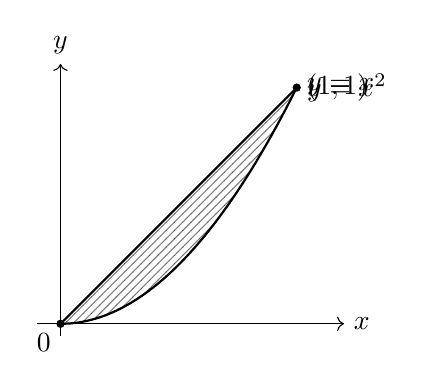
\begin{tikzpicture}[scale=3]
\draw[->] (-0.1,0)--(1.2,0) node[right] {$x$};
\draw[->] (0,-0.05)--(0,1.1) node[above] {$y$};
\draw[domain=0:1,smooth,thick] plot (\x,{\x}) node[right] {$y=x$};
\draw[domain=0:1,smooth,thick] plot (\x,{\x*\x}) node[right] {$y=x^2$};
\fill[pattern=north east lines,opacity=0.5] plot[domain=0:1] (\x,{\x}) -- plot[domain=1:0] (\x,{\x*\x}) -- cycle;
\fill (0,0) circle (0.5pt) node[below left] {$0$};
\fill (1,1) circle (0.5pt) node[right] {$(1,1)$};
\end{tikzpicture}
\end{center}

\subsection*{5(c)}
\begin{questionbox}
Two tailors A and B earn Rs. 150 and Rs. 200 per day respectively. Tailor A can stitch 6 shirts and 4 pants while Tailor B can stitch 10 shirts and 4 pants per day. How many days shall each work if it is desired to produce at least 60 shirts and 32 pants at minimum labour cost? Also calculate the least cost.
\end{questionbox}
\ans
Let tailor A work for $x$ days and tailor B work for $y$ days.

The constraints are
\[
6x+10y\ge 60 \quad \Rightarrow\quad 3x+5y\ge 30,
\]
\[
4x+4y\ge 32 \quad \Rightarrow\quad x+y\ge 8,
\]
\[
x\ge 0,
\qquad y\ge 0.
\]
The cost function to be minimized is
\[
C=150x+200y.
\]
The corner points of the feasible region relevant to minimum cost are obtained from the boundary lines.

Intersection of
\[
3x+5y=30,
\qquad x+y=8:
\]
from $x=8-y$,
\[
3(8-y)+5y=30
\Rightarrow 24+2y=30
\Rightarrow y=3,
\]
so
\[
x=5.
\]
Cost at $(5,3)$:
\[
C=150(5)+200(3)=750+600=1350.
\]
Other feasible boundary points give higher cost: $(10,0)$ gives Rs. $1500$ and $(0,8)$ gives Rs. $1600$.
Therefore the minimum occurs at $(5,3)$.
\final{\text{Tailor A should work 5 days and Tailor B should work 3 days. Minimum cost = Rs. 1350.}}

\begin{center}
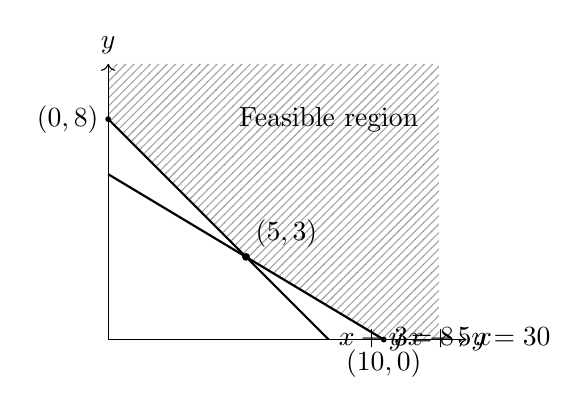
\begin{tikzpicture}[scale=0.35]
\draw[->] (0,0)--(13,0) node[right] {$x$};
\draw[->] (0,0)--(0,10) node[above] {$y$};
\draw[thick,domain=0:10] plot (\x,{(30-3*\x)/5}) node[right] {$3x+5y=30$};
\draw[thick,domain=0:8] plot (\x,{8-\x}) node[right] {$x+y=8$};
\fill[pattern=north east lines,opacity=0.35] (5,3)--(10,0)--(12,0)--(12,10)--(0,10)--(0,8)--cycle;
\fill (5,3) circle (4pt) node[above right] {$(5,3)$};
\fill (10,0) circle (3pt) node[below] {$(10,0)$};
\fill (0,8) circle (3pt) node[left] {$(0,8)$};
\node at (8,8) {Feasible region};
\end{tikzpicture}
\end{center}

\newpage
\section*{Theory and Formula Sheet}

\begin{multicols}{2}
\subsection*{Matrices}
\begin{itemize}[leftmargin=*]
\item $(A+B)^2=A^2+AB+BA+B^2$.
\item If $(A+B)^2=A^2+B^2$, then $AB+BA=O$.
\item Cramer's rule: for $AX=B$, $x_i=\Delta_i/\Delta$.
\item $A^{-1}=\dfrac{1}{|A|}\operatorname{adj}(A)$, if $|A|\ne0$.
\end{itemize}

\subsection*{Progressions}
\begin{itemize}[leftmargin=*]
\item A.P.: $T_n=a+(n-1)d$.
\item H.P.: reciprocals form an A.P.
\item G.P. finite sum: $S_n=a\dfrac{r^n-1}{r-1}$ for $r\ne1$.
\end{itemize}

\subsection*{Cube Roots of Unity}
\begin{itemize}[leftmargin=*]
\item $\omega^3=1$, $\omega\ne1$.
\item $1+\omega+\omega^2=0$.
\item Powers repeat cyclically: $\omega^{3k}=1$, $\omega^{3k+1}=\omega$, $\omega^{3k+2}=\omega^2$.
\end{itemize}

\subsection*{Complex Numbers}
\begin{itemize}[leftmargin=*]
\item If $z=x+iy$, then $|z|=\sqrt{x^2+y^2}$.
\item $\operatorname{Re}(z)=x$, $\operatorname{Im}(z)=y$.
\item Equate squared moduli to remove square roots.
\end{itemize}

\subsection*{Differentiation and Extrema}
\begin{itemize}[leftmargin=*]
\item Critical points satisfy $f'(x)=0$ or $f'(x)$ undefined.
\item First derivative test: $+$ to $-$ gives local maximum; $-$ to $+$ gives local minimum.
\item Second derivative test: $f''(a)>0$ minimum; $f''(a)<0$ maximum.
\end{itemize}

\subsection*{Integration}
\begin{itemize}[leftmargin=*]
\item Use substitution when radicals or shifted powers occur.
\item $\int \frac{du}{u}=\ln|u|+C$.
\item $\int u^n\,du=\dfrac{u^{n+1}}{n+1}+C$, $n\ne-1$.
\end{itemize}

\subsection*{Vectors and 3D Geometry}
\begin{itemize}[leftmargin=*]
\item Perpendicular vectors have zero dot product.
\item Direction cosines: $l=\frac{a}{\sqrt{a^2+b^2+c^2}}$, $m=\frac{b}{\sqrt{a^2+b^2+c^2}}$, $n=\frac{c}{\sqrt{a^2+b^2+c^2}}$.
\item Shortest distance between skew lines:
\[
D=\frac{|(\vec P_2-\vec P_1)\cdot(\vec d_1\times\vec d_2)|}{|\vec d_1\times\vec d_2|}.
\]
\end{itemize}

\subsection*{Area and Linear Programming}
\begin{itemize}[leftmargin=*]
\item Area between curves: $\int_a^b(\text{upper}-\text{lower})dx$.
\item In linear programming, optimum occurs at a corner point of the feasible region.
\item For minimization, evaluate the cost function at all relevant corner points.
\end{itemize}
\end{multicols}

\end{document}
